\documentclass[aspectratio=1610]{beamer}
\usetheme{Madrid}

\usepackage{xpatch}
\xpatchcmd{\itemize}
  {\def\makelabel}
  {\ifnum\@itemdepth=1\relax
   \setlength\itemsep{2ex}% separation for first level
   \else
   \ifnum\@itemdepth=2\relax
     \setlength\itemsep{0.5ex}% separation for second level
   \else
     \ifnum\@itemdepth=3\relax
     \setlength\itemsep{0.5ex}% separation for third level
   \fi\fi\fi\def\makelabel
  }
 {}
 {}


\usepackage{bbold}
\usepackage{setspace}

\newcommand{\st}{s.t.\ }
\newcommand{\wrt}{w.r.t.\ }
\newcommand{\eg}{e.g.\ }
\newcommand{\eq}{\ =\ }
\newcommand{\andsp}{\text{ \ \ and \ \ }}

\usepackage{amsmath}
\usepackage{bm}
\newcommand{\bb}{\mathbb}
\newcommand{\mc}{\mathcal}

\usepackage{hyperref}
\hypersetup{
  colorlinks=false,
  linkcolor=blue,
  filecolor=blue,
  urlcolor=blue,
}

\title{One and Multi-Period Asset Pricing Models}
\subtitle{\small{  \ \\
  Chapters 2, 3, 7 - Lecture Notes by Markus Brunnermeier https://scholar.princeton.edu/markus/classes/fin501
}}
\author{Presented by Yenson Lau \ | \ Layer 6 AI}
\centering
\date{April 16th, 2021}

\begin{document}
\maketitle


\begin{frame}{Today's talk}
\begin{itemize} \setlength\itemsep{1em}
\item State-space representation of security structures
\item One period setting
\item No arbitrage
\item State prices and the Fundamental Theorem of Asset Pricing
\item Pricing formulas for one period
  \begin{itemize}
    \item Stochastic discount factors (SDFs)
    \item Beta models
  \end{itemize}
\item Extension to multiple periods
\end{itemize}
\end{frame}

\begin{frame}
\huge{One-Period Asset Model}
\end{frame}

\begin{frame}{Setup}

\begin{columns}
\begin{column}{0.6\textwidth}
  \begin{itemize}
    \item {\bf Two dates:} present ($t=0$) and future ($t=1$)
    \item World is fixed at $t=0$ but has $S$ states at $t=1$
    \begin{itemize}
      \item e.g. flipping a coin, prices go up or down, S=2
    \end{itemize}
    \vspace{1ex}

    \item $p_j$: \ price of a security $j$ at $t=0$
    \item $x^j_s$: \ payoff at $t=1$ for state $s$
    \vspace{2ex}

    \item Payoff vector for asset $j$
    \begin{align*}
      \bm x^j & \eq
      \begin{bmatrix}
        x^j_1 \\
        x^j_2 \\
        \vdots \\
        x^j_S
      \end{bmatrix}
      \ \in \bb R^S
    \end{align*}

  \end{itemize}
\end{column}
\begin{column}{0.38\textwidth} \centering
  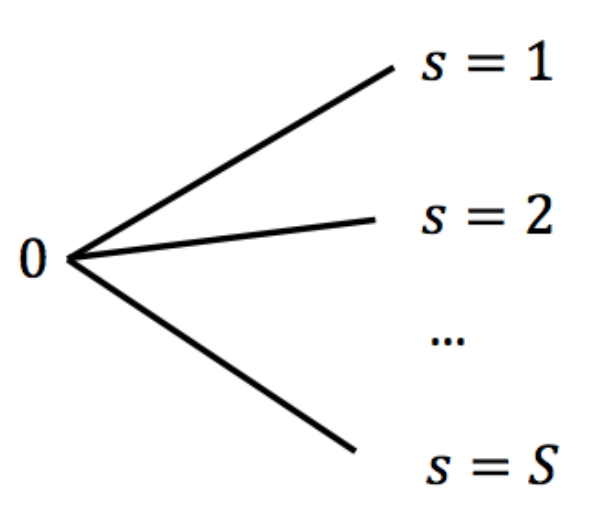
\includegraphics[width=.85\textwidth]{images/one-period.PNG}
\end{column}
\end{columns}
\end{frame}

\begin{frame}{Security Structure}
  \begin{itemize}
    \item Market consists of securities $j=1,\dots,J$
    \item A {\em security structure} $\bm X\in\bb R^{S\times J}$ is the matrix formed by concatenating payoff vectors
    $$\bm X \eq [\bm x^1, \dots, \bm x^J]$$

    \item A {\em portfolio} $\bm h = [h_1, \dots, h^j] \in \bb R^J$ denotes amount held for each of the $J$ securities
    \item The price of the portfolio is $\bm p^T \bm h$ and its payoff is $\bm{Xh}$
    \item The {\em asset span} of $\bm X$ is the set of achievable payoffs
    \begin{equation}
      \langle\bm X\rangle = \{\bm{Xh}: \bm h \in \bb R^J\}
    \end{equation}

    \item We say {\em the market is complete} if $\langle\bm X\rangle=\bb R^S$, or $\text{rank}(\bm X) = S$
  \end{itemize}
\end{frame}

\begin{frame}{Particular examples}
\begin{itemize}
  \item {\em Arrow-Debreu securities:\ } $\bm e_s = [0,\dots,1,\dots, 0]^T$, only pays off at state $s$.
  \item {\em Risk-free bonds:\ } $\bm x^b = [1, \dots, 1]$, pays off at every state.
  \item {\em Calls and puts:\ } Let $\bm x^1 = [1, 2, \dots, S]^T$. Then
  \begin{equation}
    x^k_s=\max(s+1-k,0) \quad\text{and}\quad x^k_s=\max(k-s,0), \quad k=2,\dots,S
  \end{equation}
  specify payoffs for call and put options on $\bm x^1$, respectively. Then with $\bm X = [\bm x^1, \bm x^2, \dots, \bm x^S]$
  \begin{equation}
    \bm X \eq
    \begin{bmatrix}
      1 & 0 & \dots & 0 \\
      2 & 1 & \dots & 0 \\
      \vdots & \vdots & \ddots & \vdots \\
      S & S-1 & \dots & 1
    \end{bmatrix}
    \quad \text{and} \quad
    \bm X \eq
    \begin{bmatrix}
      1 & 1 & 2 & \dots & S-1 \\
      2 & 0 & 1 & \dots & S-2 \\
      \vdots & \vdots & \vdots & \ddots & \vdots \\
      S-1 & 0 & 0 & \dots & 1 \\
      S & 0 & 0 & \dots & 0
    \end{bmatrix},
  \end{equation}
  so both call and put options can be used to construct complete markets.
\end{itemize}
\end{frame}

\begin{frame}{No Arbitrage}
\begin{itemize}
  \item {\bf Notation:}
  \begin{itemize}
    \item $y \geq x\ \implies\ y_i \geq x_i \quad \forall i$
    \item $y > x\ \implies\ y_i \geq x_i \quad \forall i$ \ \ and \ $y\neq x$ (at least 1 strict inequality)
    \item $y \gg x\ \implies\ y_i > x_i \quad \forall i$
  \end{itemize}
  \vspace{2ex}

  \item {\bf Arbitrage:\ } $\exists\, \bm h$\ \ \st \ \ $\bm p^T\bm h \leq 0$ and $\bm{Xh}\geq \bm 0$,\ \ with at least 1 strict inequality

  \item {\bf Strong arbitrage:\ } $\exists\, \bm h$\ \ \st \ \ $\bm p^T\bm h < 0$ and $\bm{Xh}\geq \bm 0$

  \item The converse can be stated as follows:
  \begin{itemize}
    \item {\bf No arbitrage (NA):\ } $\bm{Xh}>0 \implies \bm p^T\bm h > 0 \quad \forall \bm h$
    \item {\bf No strong arbitrage (NSA):\ } $\bm{Xh}\geq 0 \implies \bm p^T\bm h \geq 0 \quad \forall \bm h$
  \end{itemize}
  \vspace{2ex}

  \item NA $\implies$ NSA
\end{itemize}
\end{frame}

\begin{frame}{No Arbitrage}
\begin{itemize}
  \item {\bf Law of One Price (LOOP):\ } Any two portfolios $\bm h, \bm k \in \bb R^J$ with equal payoffs must have equal price
  $$\bm{Xh} = \bm {Xk} \ \implies \ \bm p^T \bm h = \bm p^T \bm k$$
  \item NA $\implies$ NSA $\implies$ LOOP $\implies$ every portfolio with zero payoff has zero price
  \vspace{2ex}

  \item NSA $\implies$ LOOP: \
  \begin{itemize}
    \item Contrapositive: suppose $\exists\, \bm {h,k}\ $ \st $\bm{Xh}=\bm{Xk}$, but $\bm p^T\bm h \neq \bm p^T\bm k$
    \item Then $\bm X(\bm h - \bm k) = 0$ \ but \ $\min\big(\bm p^T(\bm h - \bm k), \bm p^T(\bm k - \bm h)\big) < 0$
    \item !LOOP $\implies$ !NSA \qed
  \end{itemize}
  \item LOOP $\implies$ every portfolio with zero payoff has zero price:
  \begin{itemize}
    \item Similar to above: let $\bm{Xh}=\bm 0$ but $\bm p^T\bm h\neq 0$
    \item Setting $\bm k=\bm 0$ for LOOP leads to contrapositive\qed
  \end{itemize}
\end{itemize}
\end{frame}

\begin{frame}{State Prices}
\begin{itemize}
  \item A vector of {\em state prices}: \ $\bm q\in\bb R^S$ \ \st
  $$\bm p \eq \bm X^T\bm q \eq \sum_{s=1}^S\, q_s \cdot \bm x_s,
  \qquad \text{or} \qquad
  p_j \eq \sum_{s=1}^S q_s \cdot x^j_s \quad \forall j$$

  \item Implies all assets are discounted {\em exactly the same way} from payoffs $\bm x^j$. \\ Each state has an associated price.
  \vspace{2ex}

  \item When does such a $\bm q$ exist?
\end{itemize}

\end{frame}

\begin{frame}{Fundamental Theorem of Asset Pricing (Stiemke's Theorem)}

\vspace{5ex}
{\large A security structure $\bm X\in \bb R^{S\times J}$ provides no arbitrage opportunities
\\ iff it yields a positive state price vector.}
\vspace{5ex}

\begin{itemize}
  \item Equivalent statement: either $\exists\, \bm h \in \bb R^J$ \st
  $$\bm p^T \bm h \leq 0 \andsp \bm{Xh}\geq \bm 0$$
  with at least 1 nonzero, or $\exists\, \bm q\in \bb R^S$ \st
  $$\bm p = \bm X^T\bm q \andsp \bm q \gg \bm 0$$

  \item An example of a {\em theorem of the alternative}. Important class of theorems in convex optimization.
\end{itemize}
\end{frame}

\begin{frame}{Fundamental Theorem of Asset Pricing (Stiemke's Theorem)}
\begin{itemize}
  \item {\em Proof: \ } First we restate the alternatives as
  \begin{alignat}{3}
    &\text{I.} \quad &&\bm \exists\, \bm h \in \bb R^n: \quad
    &&\bm{Ah} > \bm 0 \\
    &\text{II.} &&\bm \exists\, \bm z \in \bb R^m:
    &&\bm A^T\bm z = \bm 0 \andsp \bm z \gg \bm 0
  \end{alignat}
  where
  \begin{equation}
    \bm A = \begin{bmatrix}
      -\bm p^T \\
      \bm X \\
    \end{bmatrix}
    \in \bb R^{m\times n} \andsp
    \bm z \propto \begin{bmatrix}
      1 \\
      \bm q \\
    \end{bmatrix}.
  \end{equation}
  \vspace{1ex}

  \item The alternatives are mutually exclusive: (II) implies $\bm h^T(\bm A^T\bm z) = 0$, but (I) implies
  $$ \bm h^T\bm A^T\bm z \eq (\bm{Ah})^T\bm z \ > \ 0.$$
\end{itemize}
\end{frame}

\begin{frame}{Fundamental Theorem of Asset Pricing (Stiemke's Theorem)}
\begin{itemize}
  \item Next assume (I) does not hold, which implies that
  \begin{equation}
    \mc S_1 = \{\bm u = \bm{Ah}: \ \bm h \in \bb R^n\}
    \andsp
    \mc S_2 = \{\bm v\in \bb R^m: \ \bm v > \bm 0\}
  \end{equation}
  are disjoint. By hyperplane separation there is a unit vector $\bm z \in \bb R^m$ \st
  \begin{equation}
    \bm z^T\bm v \ > \ 0, \ \ \forall\, \bm v \in \mc S_2
    \ \ \andsp \ \
    \bm z^T\bm{Ah} \eq 0, \ \ \forall\, \bm h\in \bb R^n.
  \end{equation}
  \item Then $\bm{A^Tz}=\bm 0$, otherwise
  \begin{equation}
    \Vert\bm A^T \bm z\Vert^2 \eq \bm z^T\bm{AA}^T\bm z \ > \ 0
  \end{equation}
  but this contradictions the hyperplane condition for $\mc S_1$ (set $\bm h = \bm A^T\bm z$).
  \item Finally show $\bm z \gg 0$: All the basis vectors of $\bb R^m$ are in $\mc S_2$.
  \\ The hyperplane condition then implies all coordinates of $\bm z$ must be positive. \qed
\end{itemize}
\end{frame}

\begin{frame}{State Prices in Incomplete Markets}
\begin{itemize}
  \item In general there can be multiple $\bm q$s, e.g.\ if $J<S$.
  \item However there is a unique $\bm q^*$ in $\langle\bm X\rangle$, known as the {\em pricing kernel}. For  instance,
  \begin{equation}
    \bm X^T(\bm X\bm u) = \bm p
  \end{equation}
  provides a unique solution for $\bm q^*=\bm{Xu}$ as long as the $\bm x^j$s are linearly independent. Furthermore, for any valid $\bm q$,
  \begin{equation}
    \bm q^* = \text{proj\,}(\bm q \, \vert\, \langle \bm X\rangle).
  \end{equation}

  \item Finally, there exists a unique $\bm q\gg0$ iff markets are complete and there is no arbitrage.
  \begin{itemize}
    \item $\impliedby$ Just solve $\bm X^T\bm q = \bm p$.
    \item $\implies$ If markets are not complete but there is no arbitrage, then $\exists\, \bm v \neq \bm 0$ \st $\bm X^T\bm v = \bm 0$.
    \\ Moreover we can find $\bm q\gg \bm 0$ and some $\alpha\in\bb R$ \st
    $$\bm q + \alpha \bm v \ \gg \ 0.$$
    So there are infinitely many solutions to $\bm X^T\bm q = \bm p$. Contrapositive. \qed
  \end{itemize}
\end{itemize}
\end{frame}

\begin{frame}{One-Period Asset Pricing: Stochastic Discount Factor (SDF)}
\begin{itemize}
  \item Discounted price if no arbitrage: $p_j = \bm q^T\bm x^j$

  \item Introduce state probabilities $\pi_s$ and {\bf stochastic discount factor (SDF)} $m_s = \frac{q_s}{\pi_s}$ (state price per unit probability)
  \begin{equation}
    p_j \eq \sum_{s=1}^S \pi_s\, \frac{q_s}{\pi_s}\, x^j_s
    \eq \sum_s \pi_s m_s x^j_s \eq \bb E[\bm m \odot \bm x^j]
  \end{equation}

  \item Consider a risk-free bond with $\bm x^b = \bm 1$. Since $\bb E[\bm m \odot \bm x^j] = \bb E[\bm m]\, \bb E[\bm x^j] + Cov(\bm m, \bm x^j)$,
  \begin{equation}
    p_b = \bb E [\bm m] = 1/R^f \quad \implies \quad
    p_j = \frac{\bb E[\bm x^j]}{R^f} + Cov[\bm m, \bm x^j]
  \end{equation}
  and for any asset $j$.

  \item Since prices tend to grow over time, typically $Cov[\bm m, \bm x^j]<0$.

\end{itemize}

\end{frame}

\begin{frame}{One-Period Asset Pricing: Stochastic Discount Factor (SDF)}
\begin{itemize}
  \item Define the return of asset $j$ as $\bm R^j\doteq\bm x^j/p_j,$
  then $\bb E\big[\bm m \odot \bm R^j\big] = 1$.
  \item Moreover, since $R^f = 1/\bb E[\bm m]$,
  \begin{equation}
    \bb E\Big[\bm m \odot \big(\bm R^j - R^f\big)\Big] \eq
    \bb E[\bm m]\, \Big(\bb E\big[\bm R^j\big] - R^f\Big)
    + Cov(\bm m, \bm R^j) \eq 0
  \end{equation}

  \item Or
  \begin{equation}
    \bb E\big[\bm R^j\big] - R^f = -\frac{Cov(\bm m, \bm R^j)}{\bb E[\bm m]}
  \end{equation}

  \item The excess return for a generic asset $j$ is determined solely by its covariance with the SDF. Investors are only compensated for holding {\em systematic risk}.

\end{itemize}
\end{frame}

\begin{frame}{Relationship to security market line / CAPM}
\begin{itemize}
  \item Consider the unique SDF $\bm m^* = [q^*_1/\pi_1,\ \dots,\ q^*_S/\pi_S]^T$
  \item Treat $\bm m^*$ as a payoff vector with price $p_{m^*}>0$. We can define $\bm R^* = \bm m^*/p_{m^*}$ and write
  \begin{equation}\label{eq:beta}
    \bb E[\bm R^j] - R^f
    \eq -\frac{Cov(\bm R^*, \bm R^j)}{\bb E[\bm R^*]}
    \eq -\ \underset{\beta_j}{\underbrace{\frac{Cov(\bm R^*, \bm R^j)}{Var(\bm R^*)}}} \cdot \frac{Var(\bm R^*)}{\bb E[\bm R^*]}
  \end{equation}

  \item By plugging in $\bb R^* \rightarrow \bb R^j$ to \eqref{eq:beta}, we get $\bb E[\bm R^*] - R^f = -Var(\bm R^*)/\bb E[\bm R^*]$, and
  \begin{equation}
    \bb E[\bm R^j] - R^f \eq \beta_j\left(\bb E[\bm R^*] - R^f \right).
  \end{equation}

  \item It remains to show that $\bm m^*$ corresponds to the payoff of the market portfolio.
\end{itemize}
\end{frame}

\begin{frame}
\begin{columns}
\begin{column}{0.58\textwidth} \centering
  \huge{Multi-Period Asset Model}
\end{column}
\begin{column}{0.4\textwidth}
  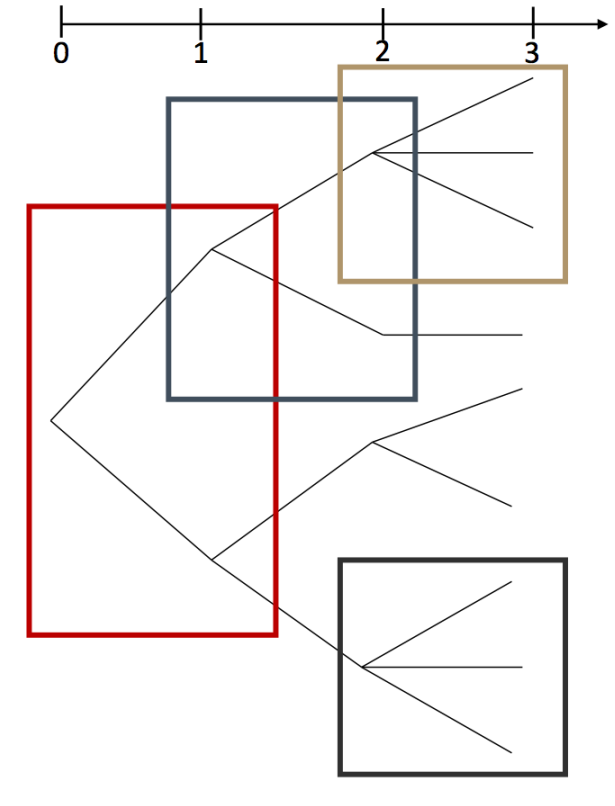
\includegraphics[height=0.85\textheight]{images/multi-period.PNG}
\end{column}
\end{columns}
\end{frame}

\begin{frame}{Dynamic Trading and Model Completeness}
\begin{columns}
\begin{column}{0.68\textwidth}
  \begin{itemize}
    \item $T$ periods. Look at each branch as a one-period setting
    \item Even if with limited assets, we can trade at each time-period to achieve completeness
    \item {\em Short-lived assets} only pays out at the period after purchase.
      \ Need $T$ assets for completeness.
      \\ First replicate an asset bought at $t=0$ and pays \$1 at $s_{2,2}$
    \begin{itemize}
      \item Arrow security: costs \$1, pays \$1 for a specific next state
      \item $q_{2,2}$: state price for $s_{2,2}$
      \item $\implies$ $q_{2,2}$ Arrow securities are needed when $A_{1,1}$ occurs
      \item To get \$1 at $A_{1,1}$, need $q_{1,1}$ Arrow securities at $t=0$
      \item $\implies$ Buy $q_{1,1}q_{2,2}$ Arrow securities at $t=0$, use payoff to purchase $q_{2,2}$ Arrow securities at $t=1$
    \end{itemize}
    Repeat for other states to establish completeness
  \end{itemize}
\end{column}
\begin{column}{0.3\textwidth}
  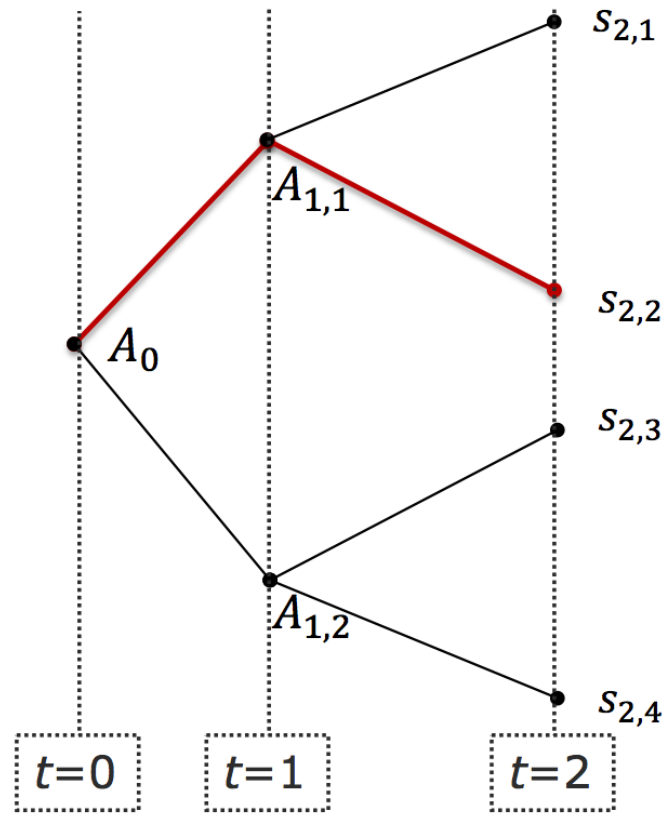
\includegraphics[width=\textwidth]{images/short-lived.PNG}
\end{column}
\end{columns}
\end{frame}

\begin{frame}{Dynamic Trading and Model Completeness}
\begin{columns}
\begin{column}{0.6\textwidth}
  \begin{itemize}
    \item {\em Long-lived assets} pay off over many time periods. Can be traded any time.
    \item Example: Two assets paying off at $t=2$.
    \begin{itemize}
      \item {\em Trading strategy} $[j,A_{t,i}]$: the cash flow of asset $j$ purchased in event $A_{t,i}$ and sold one period later.
      \item $p^j_{t,i}$: price of asset $j$ at time and state $t,i$
      \item Enumerating strategies creates payoff matrix
    \end{itemize}
    \vspace{1ex}
    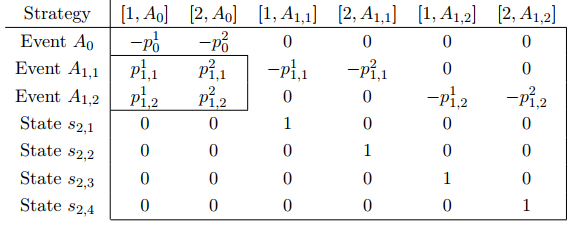
\includegraphics[width=.85\textwidth]{images/trading-strategy.PNG}
  \end{itemize}
\end{column}
\begin{column}{0.38\textwidth}
  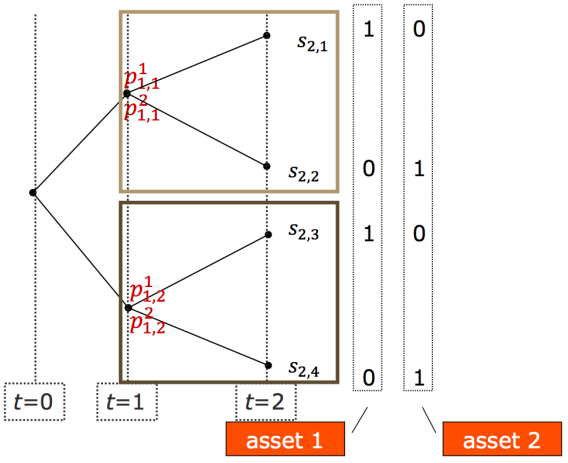
\includegraphics[width=\textwidth]{images/long-lived.PNG}
\end{column}
\end{columns}
\end{frame}

\begin{frame}{Dynamic Trading and Model Completeness}
\begin{columns}
\begin{column}{0.6\textwidth}
  \begin{itemize}
    \item Example contd.
    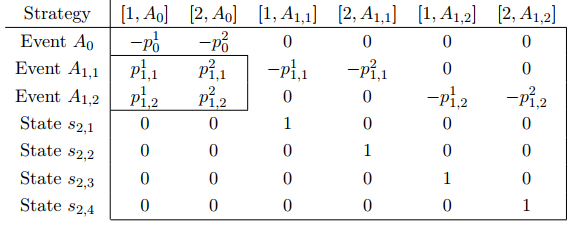
\includegraphics[width=.85\textwidth]{images/trading-strategy.PNG}
    \begin{itemize}
      \item The payoff matrix has full rank iff the highlighted submatrix has full rank
      \item {\em Generically}, the markets are {\em dynamically} complete
    \end{itemize}
    \item Generically the {\em branching number} of the tree determines assets needed for completeness
    \begin{itemize}
      \item e.g. binomial tree $\implies$ Black-Scholes, 2 assets
    \end{itemize}
  \end{itemize}
\end{column}
\begin{column}{0.38\textwidth}
  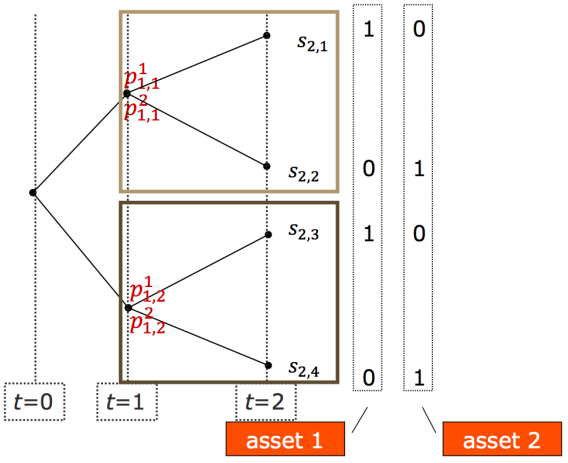
\includegraphics[width=\textwidth]{images/long-lived.PNG}
\end{column}
\end{columns}
\end{frame}

\begin{frame}{Stochastic Discount Factors}
\begin{flushleft}
  \em Some changes to notation:
  \vspace{-1ex}
\end{flushleft}
\begin{itemize}
  \item For an asset, replace $\bm x \rightarrow p_{t+1} + x_{t+1}$ \ and \ $\bm m \rightarrow m_{t+1}$
  \begin{itemize}
    \item need to keep track of the prices $p_t$ at each time
    \item $x_t$ represents deviation from price
  \end{itemize}
  \item Both $\{x_t\}_{t=0}^T$ and $\{m_t\}_{t=0}^T$ are {\em random processes}
  \begin{itemize}
    \item $x_t$ and $m_t$ are random variables over some state space $\Omega$
    \\ (e.g. corresponding directly to stock price fluctuations)
  \end{itemize}
  \item Each $x_t$ and $m_t$ measurable \wrt algebra $\mc F_t$ of the state space $\Omega$
  \item Furthermore $\{\mc F_t\}_{t=0}^T$ is a filtration: $\mc F_u \subseteq \mc F_v$ if $u \leq v$.
  \begin{itemize}
    \item Uncertainty increases over time; cannot know the future
  \end{itemize}
\end{itemize}
\end{frame}

\begin{frame}{Multi-period Stochastic Discount Factors}
\begin{itemize}
  \item One-period pricing becomes
  \begin{equation}
    p_t = \bb E_t\left[m_{t+1}\cdot(p_{t+1} + x_{t+1})\right]
  \end{equation}
  \item Multi-period SDF: \ $M_{t+1} \doteq m_1\cdot m_2 \cdot \ldots \cdot m_{t+1}$
  \item Multiplying both sides by $M_t$:
  \begin{equation}
    M_t p_t = \bb E_t\left[M_{t+1}(p_{t+1}+x_{t+1})\right]
  \end{equation}
  \item Then for $t=0$ and $t=1$,
  $$p_0 = \bb E_0\left[M_1(p_1+x_1)\right] \andsp M_1p_1 = \bb E_1\left[M_2(p_2+x_2)\right]$$
  \item Therefore
  \begin{equation}
    p_0
    \eq \bb E_0\left[\bb E_1 \left[M_2(p_2+x_2)\right] + M_1 x_1\right]
    \eq \bb E_0\left[\bb E_1 \left[M_2p_2+M_2x_2+M_1x_1\right]\right]
  \end{equation}
\end{itemize}
\end{frame}

\begin{frame}{Multi-period Stochastic Discount Factors}
  \begin{itemize}
    \item Law of Iterated Expectations: \ $\bb E_u\left[\bb E_v[X]\right] = \bb E_u[X]$ for all $\mc F_u \subseteq \mc F_v$
    \item Therefore
    \begin{equation}
      p_0
      \eq \bb E_0\left[\bb E_1 \left[M_2p_2+M_2x_2+M_1x_1\right]\right]
      \eq \bb E_0\left[M_2p_2+M_2x_2+M_1x_1\right]
    \end{equation}
    \item Iterating $k$ steps yields
    \begin{equation}
      p_0 \eq \bb E_0[M_k p_k] + \sum_{t=1}^k \bb E_0[M_tx_t]
    \end{equation}
    \item Assuming that $\lim_{k\rightarrow\infty}\bb E_0[M_kp_k] = 0$, we have
    $$p_0 = \sum_{t=1}^\infty \bb E_0[M_tx_t]$$
  \end{itemize}
\end{frame}

\begin{frame}{Some Ideas for Next Steps}
\begin{itemize}
  \item Extension to continuous time / state space
  \item Options pricing
  \item Modern derivation of portfolio theory / Black-Scholes
  \item Clarification on the multi-period setting
  \begin{itemize}
    \item Some of the notation / objects in the multi-period setting are not clearly explained
    \item Seems to be a widespread problem in financial economics literature
  \end{itemize}
  \item Multi-period SDF: crucial for pricing and represents systemic risk
  \begin{itemize}
    \item Relationship to market variables?
    \item Empirical models: Fama-French, factor models, PCA / ML models
  \end{itemize}
\end{itemize}
\end{frame}

\begin{frame}
\huge{Thanks!}
\end{frame}

\end{document}